% !TEX root = ./article.tex

\documentclass[spanish]{article}

\usepackage{mystyle}
\usepackage{myvars}
\usepackage{mylinearprogramming}



%-----------------------------

\begin{document}

	\maketitle % Insert title

	\thispagestyle{fancy} % All pages have headers and footers


%-----------------------------
%	ABSTRACT
%-----------------------------

	\begin{abstract}
		\noindent [TODO ]
	\end{abstract}

%-----------------------------
%	TEXT
%-----------------------------

	\section{Introducción}
	\label{sec:intro}

		\paragraph{}
		[TODO ]

		\subsection{Modelización Exacta}
		\label{sec:exact_formulation}

			\paragraph{}
			[TODO ]

			\begin{eqfloat}
				\begin{equation}
					\begin{array}{ll@{}ll}
						\text{Minimizar}	& \displaystyle\sum\limits_{i = 1}^{n}	\sum\limits_{j}^{n} & d_{ij}x_{ij} & \\
						\text{sujeto a}		& \displaystyle\sum\limits_{i = 0}^{n}	&	x_{ij} 	= 1, 	& \forall j \in \{1,...,n\}\\
															& \displaystyle\sum\limits_{j = 0}^{n}	&	x_{ij} 	= 1,	& \forall i \in \{1,...,n\}\\
															& \displaystyle\sum\limits_{j = 0}^{n}	&	y_{ij} - \displaystyle\sum\limits_{j = 0}^{n}	y_{ji} = -dem(i),  & \forall i \in \{1,...,n\}\\
															& \displaystyle\sum\limits_{j = 0}^{n}	&	y_{1j} - \displaystyle\sum\limits_{j = 0}^{n}	y_{j1} = -dem(i)	= \displaystyle\sum\limits_{j = 0}^{n} dem(j),  &\\
															&																				&	y_{ij} 	\leq capacity * x_{ij},  & \forall i,j \in \{0,...,n\}\\
															&                               				&	y_{ij} 	\geq 0, 	& \forall i,j \in \{1,...,n\} \\
															&                               				&	x_{ij} 	\in \{0,1\}, 	& \forall i,j \in \{1,...,n\}
					\end{array}
				\end{equation}
				\caption{Formulación estándar para el \emph{problema del viajante (TSP)}.}
				\label{eq:tsp_basic}
			\end{eqfloat}

		\subsection{Heurística de Clarke y Wright}
		\label{sec:clarke_wright}

			\paragraph{}
			[TODO ]

			\begin{figure}
	      \centering
	      \BVerbatimInput{code/clarke-wright.pseudo}
	      \caption{Heurística de \emph{Heurística de Clarke y Wright}}
	      \label{code:clarke_wright}
	    \end{figure}

	\section{Resolución de Problemas}

		\paragraph{}
		En esta sección se presentan los resultados obtenidos tras resolver el \emph{problema de enrutamiento de vehículos capacitado} (CVPR) sobre distintos conjuntos de datos de entrada. Dichos resultados se han agrupado por problema en lugar de por estrategia de resolución, lo cual permite comparar de manera más simple cada una de ellas. En algunos casos estos conjuntos de datos se corresponden con coordenadas cartesianas, para lo cual es necesario calcular la distancias entre cada par de puntos. La ventaja de la representación mediante coordenadas es la posibilidad de representación gráfica de la solución. Sin embargo, en otros casos tan solo se suministran las distancias, por lo que la representación gráfica no es posible.

		\paragraph{}
		Estos problemas han sido resueltos a partir de las dos estrategias descritas en la sección anterior, es decir, mediante su modelo exacto (utilizando la herramienta de resolución de problemas de programación lineal \emph{Xpress-Mosel}\cite{tool:xpress-mosel} restringiendo la ejecución a 100 segundos) y mediante la heurística de \emph{Clarke-Right} implementada de forma manual en dicho lenguaje.


		\subsection{Residuos}

			\paragraph{}
			El conjunto de datos está formado por la matriz de distancias entre $13$ nodos, refiriendose el primero de ellos al nodo fuente u origen. Además se proporciona la demanda del resto de nodos junto con la capacidad máxima para cada vehículo ($6000$ unidades). En este caso se ha resulto de manera exacta mediante la formulación descrita en la sección \ref{sec:exact_formulation} y de manera aproximada a partir de la heurística de \emph{Clarke-Wright} mediante la implementación que se muestra en la sección \ref{sec:clarke_wright}. Los resultados se muestran en la tabla \ref{table:sol-residuos}.


			\begin{table}[h]
				\centering
				\begin{tabu}{ | c | c | c | p{.58\linewidth} |}
					\hline
					\bfseries Método & \bfseries Vehículos  & \bfseries Distancia & \bfseries Caminos
					\csvreader[head to column names]{../results/csv/residuos.csv}{}
					{\\\hline\method&\vehicles&\distance&\path}
					\\\hline
				\end{tabu}
				\caption{Resultados para el \emph{problema de rutado de vehículos capacitado (CVRP)} sobre el conjunto de datos \emph{Residuos}}
				\label{table:sol-residuos}
			\end{table}

		\subsection{Gasóleos}

			\paragraph{}
			El conjunto de datos está formado por la matriz de distancias entre $7$ nodos, refiriendose el primero de ellos al nodo fuente u origen. Además se proporciona la demanda del resto de nodos junto con la capacidad máxima para cada vehículo ($39000$ unidades). En este caso se ha resulto de manera exacta mediante la formulación descrita en la sección \ref{sec:exact_formulation} y de manera aproximada a partir de la heurística de \emph{Clarke-Wright} mediante la implementación que se muestra en la sección \ref{sec:clarke_wright}. Los resultados se muestran en la tabla \ref{table:sol-gasoleos}.


			\begin{table}[h]
				\centering
				\begin{tabu}{ | c | c | c | p{.58\linewidth} |}
					\hline
					\bfseries Método & \bfseries Vehículos  & \bfseries Distancia & \bfseries Caminos
					\csvreader[head to column names]{../results/csv/gasoleos.csv}{}
					{\\\hline\method&\vehicles&\distance&\path}
					\\\hline
				\end{tabu}
				\caption{Resultados para el \emph{problema de rutado de vehículos capacitado (CVRP)} sobre el conjunto de datos \emph{Gasóleos}}
				\label{table:sol-gasoleos}
			\end{table}


		\subsection{E021-04m}

			\paragraph{}
			El conjunto de datos está formado por las coordenadas referidas a $21$ nodos, refiriendose el primero de ellos al nodo fuente u origen. Además se proporciona la demanda del resto de nodos junto con la capacidad máxima para cada vehículo ($85$ unidades) así como el número mínimo de ellos ($4$ vehículos) para resolver el problema. En este caso se ha resulto de manera exacta mediante la formulación descrita en la sección \ref{sec:exact_formulation} y de manera aproximada a partir de la heurística de \emph{Clarke-Wright} mediante la implementación que se muestra en la sección \ref{sec:clarke_wright}. Los resultados se muestran en la tabla \ref{table:sol-e021-04m}. Puesto que en este caso los datos se refieren a un problema euclídeo (con coordenadas) la representación gráfica de las soluciones se muestran en la figura \ref{fig:sol-e021-04m}.


			\begin{figure}[h]
				\centering
				\begin{subfigure}{.4\textwidth}
					\centering
					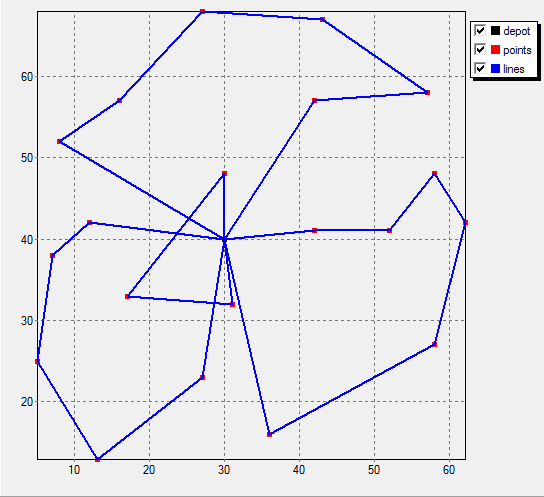
\includegraphics[width=\linewidth]{E021-04m-exact}
					\caption{Solución \emph{Exacta}}
				\end{subfigure} \
				\begin{subfigure}{.4\textwidth}
					\centering
					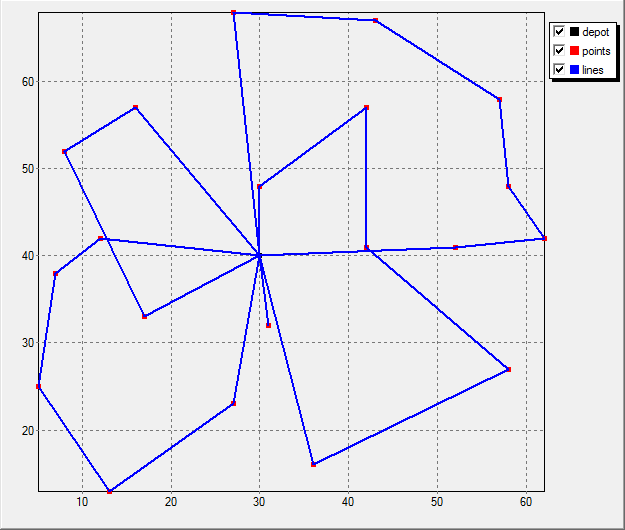
\includegraphics[width=\linewidth]{E021-04m-clarke-wright}
					\caption{Solución \emph{Clarke y Wright}}
				\end{subfigure}
				\caption{Resultados para el \emph{problema de rutado de vehículos capacitado (CVRP)} sobre el conjunto de datos \emph{E021-04m}}
				\label{fig:sol-e021-04m}
			\end{figure}

			\begin{table}[h]
				\centering
				\begin{tabu}{ | c | c | c | p{.58\linewidth} |}
					\hline
					\bfseries Método & \bfseries Vehículos  & \bfseries Distancia & \bfseries Caminos
					\csvreader[head to column names]{../results/csv/e021-04m.csv}{}
					{\\\hline\method&\vehicles&\distance&\path}
					\\\hline
				\end{tabu}
				\caption{Resultados para el \emph{problema de rutado de vehículos capacitado (CVRP)} sobre el conjunto de datos \emph{E021-04m}}
				\label{table:sol-e021-04m}
			\end{table}


		\subsection{E026-08m}

			\paragraph{}
			El conjunto de datos está formado por las coordenadas referidas a $26$ nodos, refiriendose el primero de ellos al nodo fuente u origen. Además se proporciona la demanda del resto de nodos junto con la capacidad máxima para cada vehículo ($48$ unidades) así como el número mínimo de ellos ($8$ vehículos) para resolver el problema. En este caso se ha resulto de manera exacta mediante la formulación descrita en la sección \ref{sec:exact_formulation} y de manera aproximada a partir de la heurística de \emph{Clarke-Wright} mediante la implementación que se muestra en la sección \ref{sec:clarke_wright}. Los resultados se muestran en la tabla \ref{table:sol-e026-08m}. Puesto que en este caso los datos se refieren a un problema euclídeo (con coordenadas) la representación gráfica de las soluciones se muestran en la figura \ref{fig:sol-e026-08m}.

			\begin{figure}[h]
				\centering
				\begin{subfigure}{.4\textwidth}
					\centering
					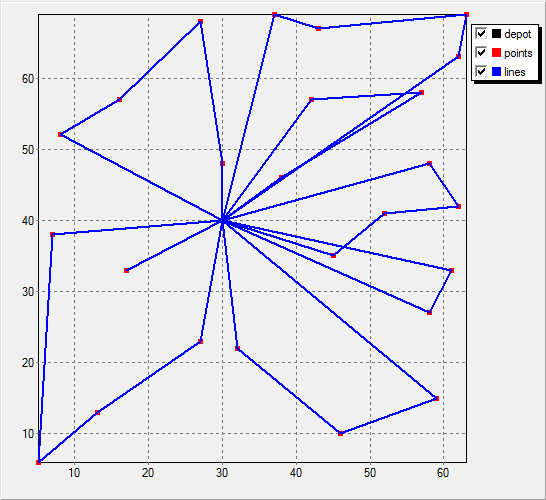
\includegraphics[width=\linewidth]{E026-08m-exact}
					\caption{Solución \emph{Exacta}}
				\end{subfigure} \
				\begin{subfigure}{.4\textwidth}
					\centering
					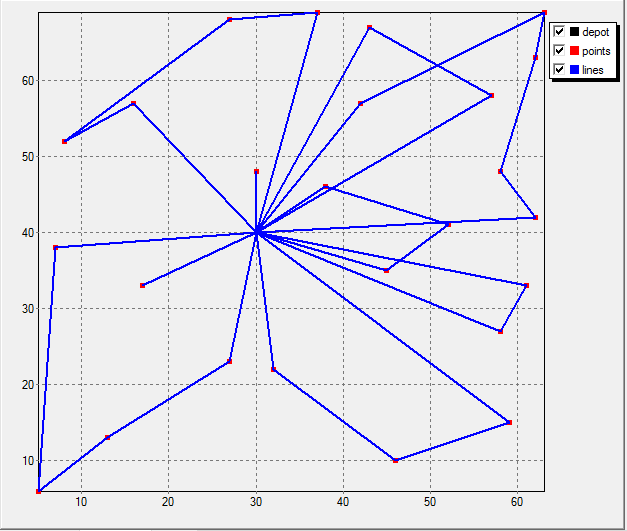
\includegraphics[width=\linewidth]{E026-08m-clarke-wright}
					\caption{Solución \emph{Clarke y Wright}}
				\end{subfigure}
				\caption{Resultados para el \emph{problema de rutado de vehículos capacitado (CVRP)} sobre el conjunto de datos \emph{E026-08m}}
				\label{fig:sol-e026-08m}
			\end{figure}

			\begin{table}[h]
				\centering
				\begin{tabu}{ | c | c | c | p{.58\linewidth} |}
					\hline
					\bfseries Método & \bfseries Vehículos  & \bfseries Distancia & \bfseries Caminos
					\csvreader[head to column names]{../results/csv/e026-08m.csv}{}
					{\\\hline\method&\vehicles&\distance&\path}
					\\\hline
				\end{tabu}
				\caption{Resultados para el \emph{problema de rutado de vehículos capacitado (CVRP)} sobre el conjunto de datos \emph{E026-08m}}
				\label{table:sol-e026-08m}
			\end{table}

		\subsection{E051-05e}

			\paragraph{}
			El conjunto de datos está formado por las coordenadas referidas a $51$ nodos, refiriendose el primero de ellos al nodo fuente u origen. Además se proporciona la demanda del resto de nodos junto con la capacidad máxima para cada vehículo ($160$ unidades) así como el número mínimo de ellos ($5$ vehículos) para resolver el problema. En este caso se ha resulto de manera exacta mediante la formulación descrita en la sección \ref{sec:exact_formulation} y de manera aproximada a partir de la heurística de \emph{Clarke-Wright} mediante la implementación que se muestra en la sección \ref{sec:clarke_wright}. Los resultados se muestran en la tabla \ref{table:sol-e051-05e}. Puesto que en este caso los datos se refieren a un problema euclídeo (con coordenadas) la representación gráfica de las soluciones se muestran en la figura \ref{fig:sol-e051-05e}.


			\begin{figure}[h]
				\centering
				\begin{subfigure}{.4\textwidth}
					\centering
					\includegraphics[width=\linewidth]{e051-05e-exact}
					\caption{Solución \emph{Exacta}}
				\end{subfigure} \
				\begin{subfigure}{.4\textwidth}
					\centering
					\includegraphics[width=\linewidth]{e051-05e-clarke-wright}
					\caption{Solución \emph{Clarke y Wright}}
				\end{subfigure}
				\caption{Resultados para el \emph{problema de rutado de vehículos capacitado (CVRP)} sobre el conjunto de datos \emph{E051-05e}}
				\label{fig:sol-e051-05e}
			\end{figure}

			\begin{table}[h]
				\centering
				\begin{tabu}{ | c | c | c | p{.58\linewidth} |}
					\hline
					\bfseries Método & \bfseries Vehículos  & \bfseries Distancia & \bfseries Caminos
					\csvreader[head to column names]{../results/csv/e051-05e.csv}{}
					{\\\hline\method&\vehicles&\distance&\path}
					\\\hline
				\end{tabu}
				\caption{Resultados para el \emph{problema de rutado de vehículos capacitado (CVRP)} sobre el conjunto de datos \emph{E051-05e}}
				\label{table:sol-e051-05e}
			\end{table}

		\subsection{E076-10e}

			\paragraph{}
			El conjunto de datos está formado por las coordenadas referidas a $76$ nodos, refiriendose el primero de ellos al nodo fuente u origen. Además se proporciona la demanda del resto de nodos junto con la capacidad máxima para cada vehículo ($140$ unidades) así como el número mínimo de ellos ($10$ vehículos) para resolver el problema. En este caso se ha resulto de manera exacta mediante la formulación descrita en la sección \ref{sec:exact_formulation} y de manera aproximada a partir de la heurística de \emph{Clarke-Wright} mediante la implementación que se muestra en la sección \ref{sec:clarke_wright}. Los resultados se muestran en la tabla \ref{table:sol-e076-10e}. Puesto que en este caso los datos se refieren a un problema euclídeo (con coordenadas) la representación gráfica de las soluciones se muestran en la figura \ref{fig:sol-e076-10e}.


			\begin{figure}[h]
				\centering
				\begin{subfigure}{.4\textwidth}
					\centering
					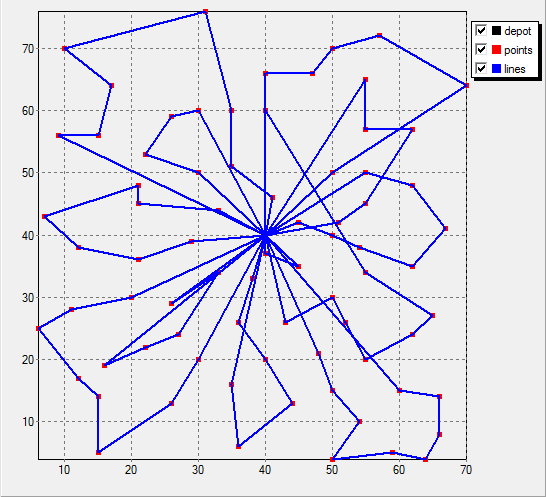
\includegraphics[width=\linewidth]{E076-10e-exact}
					\caption{Solución \emph{Exacta}}
				\end{subfigure} \
				\begin{subfigure}{.4\textwidth}
					\centering
					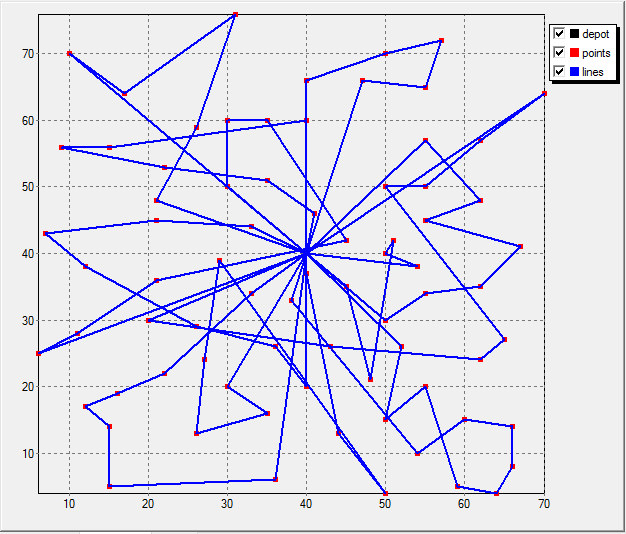
\includegraphics[width=\linewidth]{E076-10e-clarke-wright}
					\caption{Solución \emph{Clarke y Wright}}
				\end{subfigure}
				\caption{Resultados para el \emph{problema de rutado de vehículos capacitado (CVRP)} sobre el conjunto de datos \emph{E076-10e}}
				\label{fig:sol-e076-10e}
			\end{figure}

			\begin{table}[h]
				\centering
				\begin{tabu}{ | c | c | c | p{.58\linewidth} |}
					\hline
					\bfseries Método & \bfseries Vehículos  & \bfseries Distancia & \bfseries Caminos
					\csvreader[head to column names]{../results/csv/e076-10e.csv}{}
					{\\\hline\method&\vehicles&\distance&\path}
					\\\hline
				\end{tabu}
				\caption{Resultados para el \emph{problema de rutado de vehículos capacitado (CVRP)} sobre el conjunto de datos \emph{E076-10e}}
				\label{table:sol-e076-10e}
			\end{table}

%-----------------------------
%	BIBLIOGRAPHY
%-----------------------------
	\nocite{subject:mio}
	\nocite{garciparedes:mosel-examples}
	\bibliographystyle{alpha}
  \bibliography{bib/misc}

\end{document}
